\section{Quick Sort}
Supponiamo di dover ordinare la sequenza di numeri\\[12pt]
{\texttt{44 55 12 42 94 6 18 67}}\\[12pt]
Scegliamo all'interno di essa un qualunque elemento, ad esempio {\texttt{42}}
(che chiameremo {\emph{perno}} o {\emph{pivot}}), e costruiamo due sequenze nelle quali collochiamo
rispettivamente tutti gli elementi minori o uguali al perno e tutti quelli maggiori, in qualunque ordine:\\[12pt]
{\texttt{12 42 6 18 $\quad$ 44 55 94 67}}\\[12pt]
Ordinando separatamente le due sequenze e concatenandole otteniamo la 
sequenza ordinata:\\[12pt]
{\texttt{6 12 18 42 44 55 67 94}}\\[12pt]

\begin{figure}[h]
    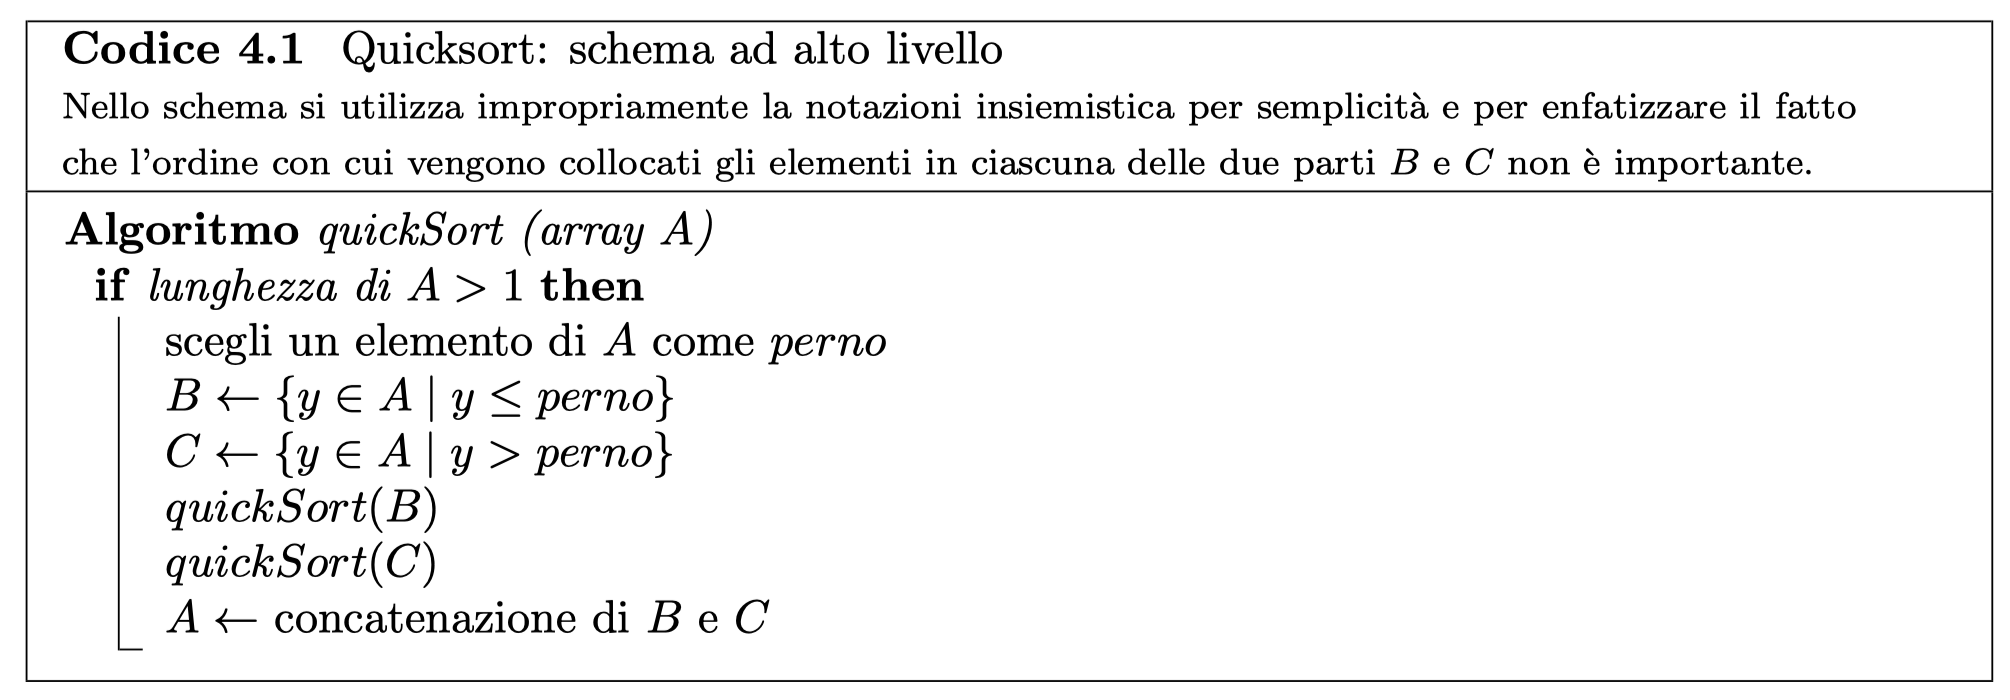
\includegraphics[width=\textwidth]{quicksortal.png}
\end{figure}

\subsection{Partiziona}

Per creare la partizione dell'array procediamo nel seguente modo:
\begin{enumerate}
    \item Scegliamo come perno l'elemento più a sinistra dell'array
    \item Scansioniamo l'array da destra verso sinistra fino al primo elemento minore o uguale al perno
    \item Scansioniamo l'array da sinistra verso destra fino al primo elemento maggiore del perno
    \item Se le due scansioni non si sono incontrate, scambiamo i due elementi individuati e proseguiamo le scansioni ai passi 2 e 3
    \item Quando ogni elemento è stato confrontato con il perno, scambiamo il perno con l'elemento su cui si è arrestata la scansione da destra 
\end{enumerate}

\noindent
Per le scansioni da destra e da sinistra utilizziamo due indici di nome 
$dx$ e $sx$, che indicano gli elementi correntemente ispezionati dalle due scansioni.
Ad ogni passo tutti gli elementi a sinistra dell'indice $sx$ risultano minori 
o uguali al perno, mentre quelli a destra di $dx$ maggiori del perno. Quando i due indici
si incontrano o $sx \ge dx$ tutti gli elementi sono stati ispezionati.
Inoltre, l'elemento di indice $dx$ è minore o uguale al perno. A questo punto
è sufficiente scambiare questo elemento con il perno per ottenere la partizione.

\begin{figure}[h]
    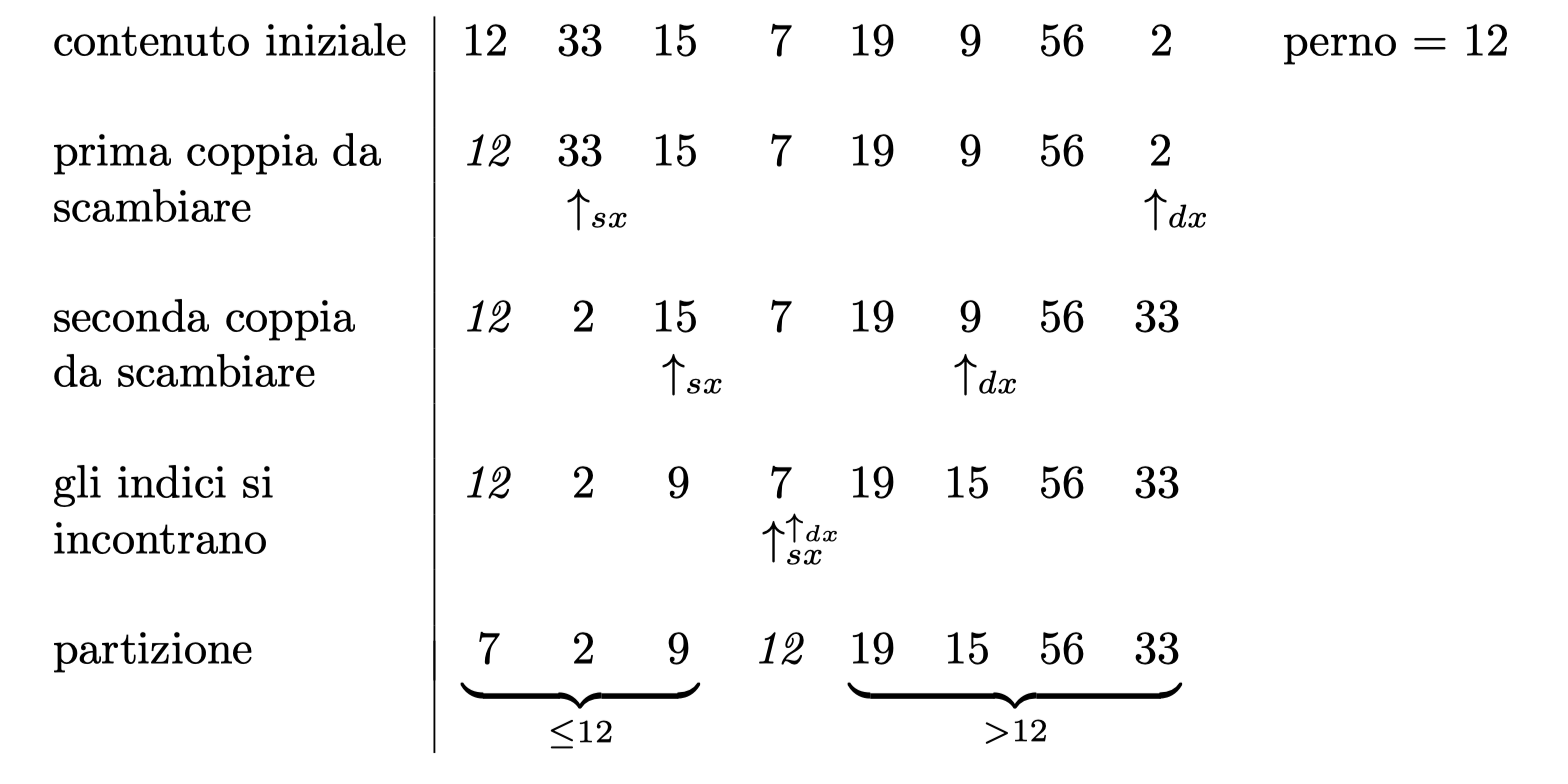
\includegraphics[width=\textwidth]{espartizione.png}
\end{figure}

\begin{figure}[h]
    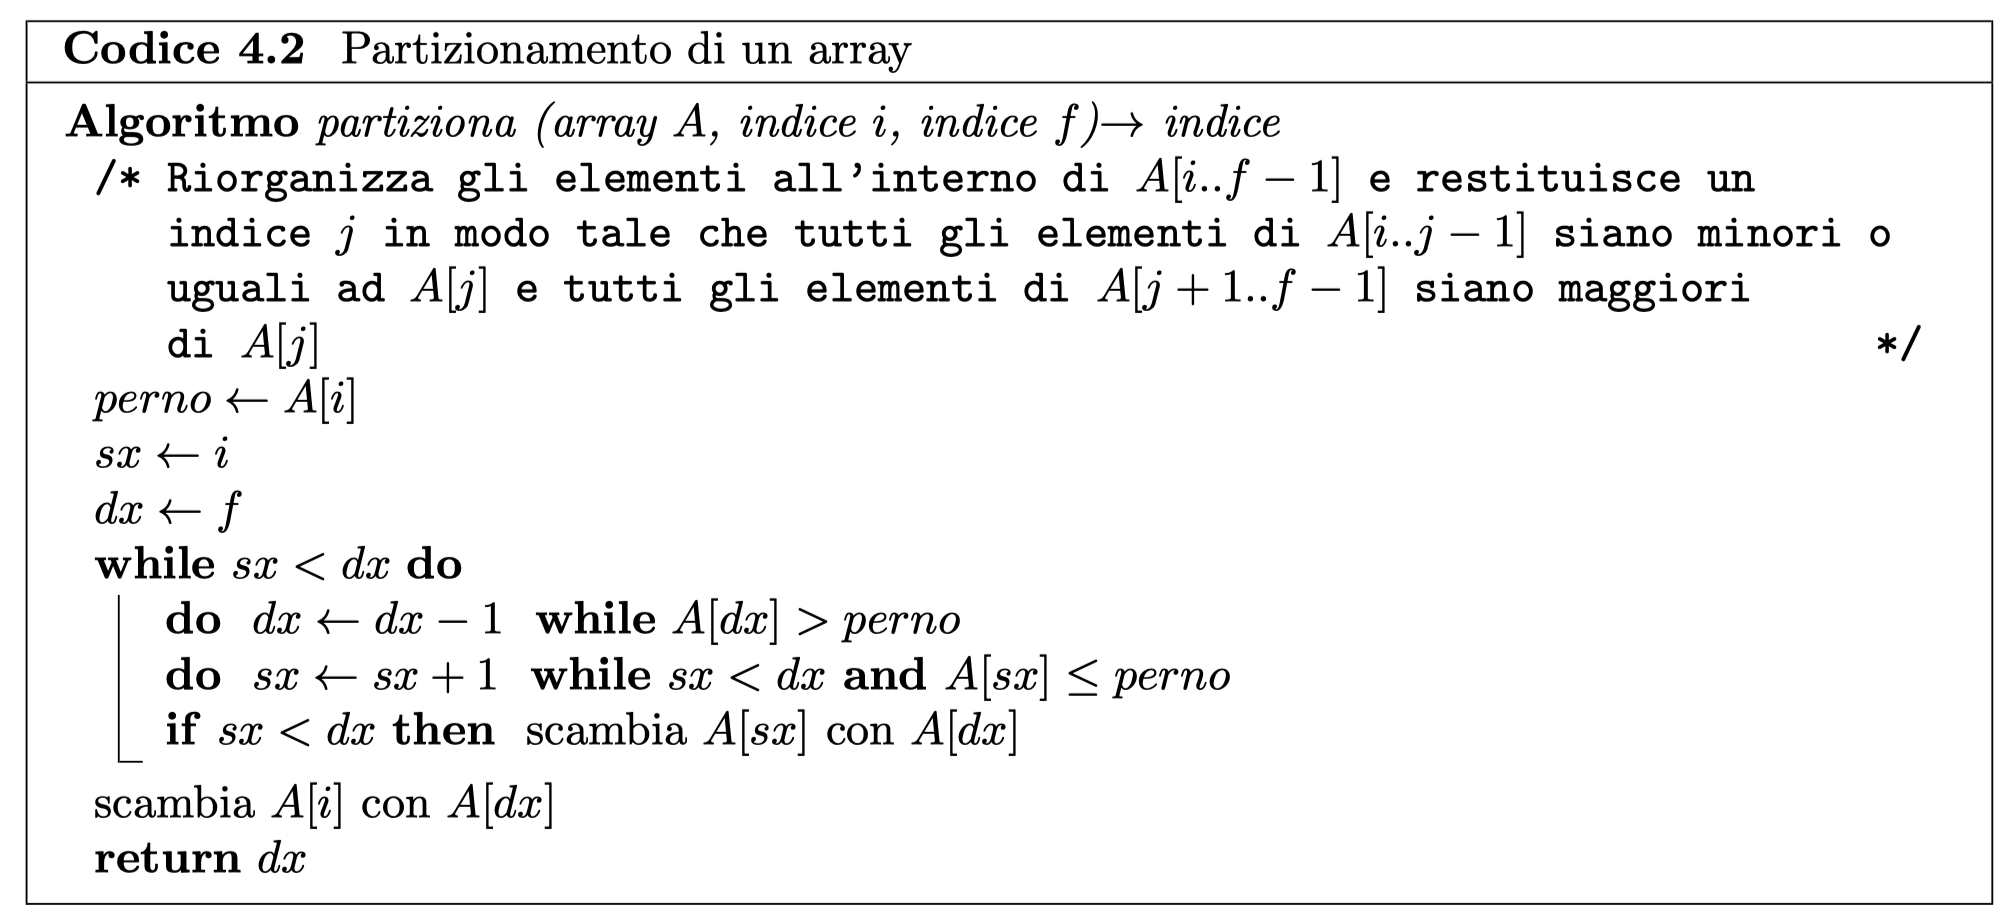
\includegraphics[width=\textwidth]{partiziona.png}
\end{figure}
\clearpage

\subsection*{Numero di confronti}

\begin{figure}[h]
    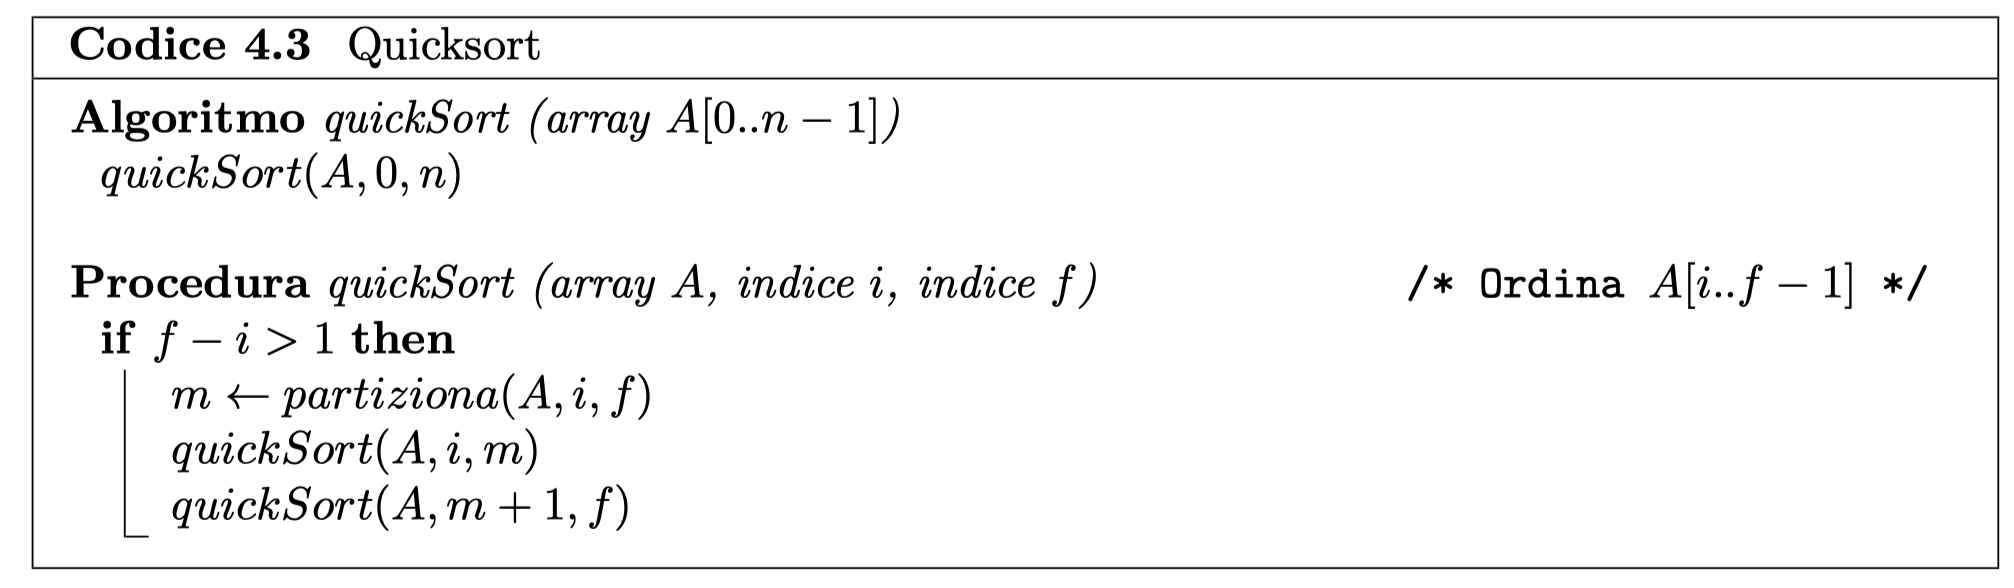
\includegraphics[width=\textwidth]{quicksort.png}
\end{figure}

Per effettuare la partizione ogni elemento dell'array deve essere confrontato con il perno
(eccetto il perno stesso). Pertanto vi sono almeno $n - 1$ confronti. Per semplicità di calcolo
utilizzeremo solo $n$\\

\subsubsection*{Caso peggiore}
Nel caso peggiore $C_{w}(n)$ {\texttt{quickSort}} esegue il seguente numero di confronti:
\begin{equation*}
    C_{w}(n) = \begin{cases}
        n + max{C_{w}(n) + C_{w}(n-k-1) | 0 \le k \le n} & \text{se $n > 1$}\\
        0 & \text{altrimenti}
    \end{cases}
\end{equation*}
Il secondo addendo della somma rappresenta il numero di confronti nelle chiamate 
ricorsive nell'ipotesi che, dopo la partizione, vi siano $k$ elementi a sinistra
del perno e $n-k-1$ a destra. Dato che stiamo studiando il caso peggiore 
consideriamo il valore di $k$ che massimizza la somma. Svolgendo i calcoli otteniamo
$C_{w}(n) = \Theta(n^2)$. Pertanto nel caso peggiore (molto raro) {\texttt{quickSort}}
effettua lo stesso numero di confronti degli algoritmi elementari che abbiamo studiato.

\subsubsection*{Caso migliore}
Abbiamo visto che il caso peggiore si ottiene quando ad ogni livello della ricorsione
la partizione risulta sbilanciata. Se, al contrario, l'array viene sempre suddiviso
in due parti circa della stessa lunghezza, il numero di confronti diminuisce drasticamente.
\begin{equation*}
    C_{b}(n) = \begin{cases}
        n + 2C_{b}(n/2) & \text{se $n > 1$}\\
        0 & \text{altrimenti}
    \end{cases}
\end{equation*}

\noindent Svolgendo i calcoli otteniamo $C_{b}(n) = n \log_2 n$

\subsubsection*{Caso medio}
Il numero di confronti effettuato da {\texttt{quickSort}} dipende dalla distribuzione
dei valori all'interno dell'array. Si può calcolare che il caso medio $C(n) \le 1.39n \log_2 n$, 
molto vicino al caso migliore e a {\texttt{mergeSort}}, motivo per cui {\texttt{quickSort}}
viene utilizzato molto spesso. 

\subsubsection*{Spazio di lavoro}
L'algoritmo è in loco ma utilizza spazio aggiuntivo per la ricorsione. Ogni 
record di attivazione deve contenere i parametri $i$ ed $f$ che delimitano
la parte di array da ordinare, oltre alla variabile $m$. Dunque la grandezza
di ciascun record di attivazione è costante. La quantità di memoria utilizzata 
è proporzionale all'altezza raggiunta dallo stack, che nel caso peggiore è $n$.
Si può modificare
l'algoritmo in modo che l'altezza dello stack sia sempre $O(\log n)$ eliminando una chiamata
ricorsiva e ordinando prima la parte destra dell'array e poi la sinistra.

\subsubsection*{Alcune osservazioni}
Possiamo osservare che le prestazioni di {\texttt{quickSort}}, su uno stesso array
possono variare notevolmente in base alla strategia utilizzata per scegliere il perno.
Spesso, per evitare il caso peggiore (array già ordinato), si utilizzano strategie
"randomizzate". Una possibilità è quella di disordinare in modo casuale gli
elementi dell'array prima di eseguire l'algoritmo, un'altra può essere
scegliere un elemento casuale dell'array da usare come perno e scambiarlo con il 
primo elemento, applicando poi la strategia di partizione che abbiamo visto.
Si può osservare che questo metodo di ordinamento non è stabile. 
\clearpage